% Chapter 1

\chapter{Background} % Main chapter title

\label{Chapter1} % For referencing the chapter elsewhere, use \ref{Chapter1} 

\lhead{Chapter 1. \emph{Overview of geothermal systems}} % This is for the header on each page - perhaps a shortened title

%----------------------------------------------------------------------------------------
%\section{Introduction}
%Y-This is the introduction




\section{Hydrothermal system}
Hydrothermal systems can be defined as a set of processes that redistribute energy and mass in response to fluid circulation \cite{Norton1984}. Hydrothermal systems includes heat, fluid and sufficient permeability in the natural geological formation. The heat source is a magma chamber. Less frequently the source of heat is the crust with an abnormal high concentration of radioisotopes, mainly potassium 40, thorium 232, and uranium 235 and 230 \cite{springer}. The origin of the fluid is meteoric, that is rain water that percolates the ground, and frequently mixed with fluids and solutes of magnetic origin. In connection to geothermal energy, the most important properties of hydrothermal systems are given by rock and fluid properties. They are:
permeability, porosity and storage capacity \cite{Axelsson2008L}. The permeability represents viscous interactions between fracture surfaces and the fluid as it flows through interconnected fracture networks \cite{Norton1984}. Permeability expresses the ease at witch fluid flows through the medium. It is a qualitative property of the system, while porosity is a quantitative property described bellow.

\subsection{Hydrological properties}
the main hydrological property is porosity. Hydrothermal systems are mainly an interconnection of fracture. However, hydrothermal system can be approximated by porous medium \cite{Ax-Lecture08}.
\subsubsection{Porous medium}
A porous medium is a substance containing voids or pores, allowing fluid to be trapped or to flow throughout the medium. in the contest of geothermal energy, we are interested in the voids within the subsurface geological formation such as rock. To allow fluid flow, the pores spaces must form a network of interconnected voids space. Based on the time they were formed, the pores space can be divided in two, \cite{Bear88}. Original pore spaces are formed during the rock formation while secondary pore spaces are formed after the rock formation. Secondary porosity are due to physical and chemical changes occurring during the conversion of one rock type to an other. Porous medium can be classified based on their constituents. Intragranular porous medium created by voids within the rock grains and Intergranular porous medium formed by the voids between the rock grains. Fracture porosity is due to fractures within the rock caused by tensional forces. On the basis of mechanical properties, we can distinguish between consolidated porosity and unconsolidated porosity. In the consolidated case, the grains are kept together with a cementing material, while in the unconsolidated case the grains are loose, \cite{Bear88}. \\
Matrix porosity as a statistical measure of the voids spaces with respect to the total rock volume can be expressed as 

\begin{equation}
\Phi = \frac{V_{T}}{V_{T}} = 1-\frac{V_{S}}{V_{T}} \nonumber
\end{equation}

where 
\begin{equation}
V_{T}=V_{S}+V_{P} \nonumber
\end{equation}

is the total porosity, $V_{P}, V_{S}$ are the pore volume and solid (rock) volume respectively. In geothermal systems, only effective porosity is of importance, because it reflects interconnected pores and allow fluid to flow, \cite{Ax-Lecture08}. Effective porosity affects the storage capacity of the medium, which is its ability to absorb or release fluid in response of pressure change, due to fluid extraction or fluid injection in the medium. Alternatively we can define fracture porosity as the fraction of volume occupied by fractures.
\begin{figure}[htp] %  figure placement: here, top, bottom, or page
   \centering
   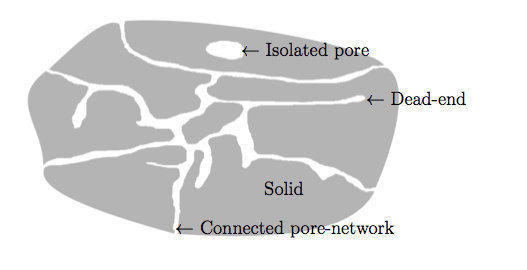
\includegraphics[width=4in]{porous.png} 
   \caption{A porous medium with connected network of pores, from \cite{Carina11}}
   \label{fig:porous}
\end{figure}

The recharge mechanism of porous medium are partly due to precipitation from the highland, that infiltrate the ground under gravity, filling up the interconnected pores spaces to form a saturation zone, \cite{Bear88}. When a part of the porous medium is trapped between impermeable formation, it is termed confined. Alternatively, an unconfined aquifer is bounded above by a water table. The movement of cold water in porous medium is described by Darcys law

\subsubsection{Darcy�s law}
Henry Darcy was a French hydraulic engineer interested in purifying water supplies using sand filters. He conducted experiments to determine the flow rate of water through the filters. Published in 1856, his conclusions have served as the basis for all modern analysis of ground water flow.The motion of cold water in porous medium is described by Darcy�s law:

\begin{equation}
Q = -K\frac{\rho}{\mu}(\Delta P-\rho g) \nonumber
\end{equation}

where 

\[
 K = \begin{bmatrix}
       K_{x} & 0 & 0           \\[0.3em]
       0 & K_{y} & 0 \\[0.3em]
       0 & 0 & K_{z}
     \end{bmatrix}
\]   
\\
\\
is the permeability tensor in 3 dimension. $Q (kg/sm^{2})$ is the fluid  flow rate, $\Delta P (Pa/m)$ the pressure gradient, $g$ acceleration of gravity and $\mu$ the fluid kinematic viscosity.  Darcy�s law stipulates that the motion of cold water in porous medium is due to the difference in pressure between two points and/or gravity forces. Capillarity pressure are pressure associated with low porosity, and can be neglected if we assume that fluid is flowing through the porous medium. Darcy�s law hold for laminar flow characterised by

\begin{equation}
R_{e}=\frac{Vd}{\nu},  \quad 1\leq R_{e} \leq 10 \nonumber
\end{equation}
where $d$ is the flow path diameter and $R_{e}$ the Reynolds number. Darcy�s law hold in porous medium but also in fracture medium, since large scale fracture medium can be approximated by porous medium, \cite{Ax-Lecture08}.
The pore velocity $v$ or the interstitial velocity is related to Darcy law by dividing the flow rate $Q$ by the porosity $\phi$. The pore velocity would be the velocity a conservative tracer would experience if carried by the fluid through the formation
\begin{equation}
v = \frac{Q}{\Phi} \nonumber
\end{equation}







\subsection{Thermal properties}
As mention before,  about $80 \%$ of the earth energy is generated by the decay of unstable  radio active elements in the crust and the mantle, \cite{Fowler05}. The major heat producing elements are  Uranium-238, Uranium-235, Potassium-40, and thorium-232 

 

\begin{table}[H]
\begin{center}
    \begin{tabular}{ | l | l | l | p{5cm} |}
    \hline
    elements & Heat generation $ (W/kg^{-1} )$ & Quatity $ (ppb) $ & Summary \\ \hline
    Uranium & $9.8.10^{-5} $& 15-25 & Uranium-238 produces $99 .28\%$ of the total Uranium energy. Uranium-235 produce $0.72\%$ of the total energy produce by Uranium. \\ \hline
    Thorium& $2.6.10^{-5}$ & 80-100 & Thorium-232 one out of $10^{4}$\\ \hline
    Potassium & $3.35.10^{19}$ & 150-260 & Potassium generate more energy  per kg. \\
    \hline
       % \caption{Heat producing radioactive elements \cite{Fowler05}}

    \end{tabular}
\end{center}
    \caption{Heat producing radioactive elements, \cite{Fowler05}}

\end{table}

The Crust generate 100 time more energy than the mantle per unit volume. However, the rate of energy generation for the entire earth is influenced by the mantle due to it large volume relatively to the crust, where the fifth of radioactive heat is generated. The total energy of the crust is about $1.4-2.7.10^{13} W$ \cite{Fowler05}. Due to low matrix and fracture  porosity, about 80 to 90$\%$ of this energy is stored in the rocks, \cite{Bod-R89}. 
%\subsubsection{Heat transfer within the earth}
The energy generated is mostly transfer through convection and  conduction. Radiation is ignored in modelling heat and mass extraction in hydrothermal systems. However, radiation plays an important role in shock wave propagation in hydrothermal systems. Hot fluid moves in the system through convective cells, where fractures are predominant. \\
consider a volume $V_{c}, V_{h}$ of cold and hot water respectively, and associated mass $m_{c}, m_{h}$. Assume that the fluid is heated bellow. The density of fluid is given by
 
\begin{equation} \label{eq:density}
\rho = \rho_{0}[1-\alpha(T-T_{0})+\beta(P-P_{0})]. \nonumber
\end{equation}
where  the compressibility 

\begin{equation}
\beta=-\frac{1}{\rho}\frac{d\rho}{dp}=-\frac{1}{V}\frac{dV}{dp} \nonumber.
\end{equation}

and $\alpha$ is the extensibility. The density decreases with increasing temperature, therefore

\begin{equation}
m_{h}=\rho_{h} V_{h} \le \rho_{c} V_{c}= m_{c}. \nonumber
\end{equation}
 
The column of hot water will rise when it is heated bellow. As it rises away from the heat source, it temperature decrease and the density of the fluid increase, allowing the column of cold water to fall. This create a convective cell. Many such cells are responsible for heat transfer in fractured porous medium. 

\begin{figure}[htp] %  figure placement: here, top, bottom, or page
   \centering
   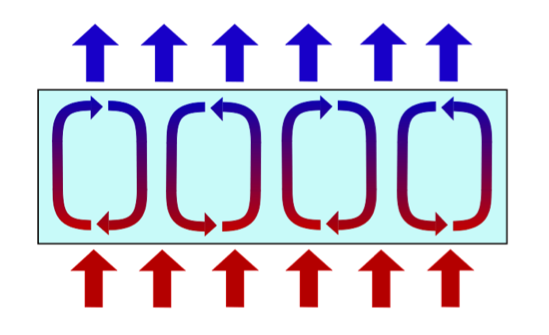
\includegraphics[width=4in]{cell.png} 
   \caption{A convective cell heated from bellow, from \cite{Carina11}}
   \label{fig:cell}
\end{figure}
When rock within the upper mantle and the crust are partially melted, the resulted molten lava, with lower density rises toward shallower depth in the form of magma chamber, dykes, or volcanics discharge, \cite{Pruess02}.\\
Conduction is predominant in sedimentary systems, where due to sediments packed together, fractures are more scarcer. in those systems, the microscopic particles undergoes constant oscillations and collisions. The energy generated by this chaotic movement create a temperature gradient causing heat to flow smoothly from region of higher temperature to region of low temperature. This is expressed by Fourier law
\begin{equation}
q = -k\Delta T
\end{equation} 
where $q, k, T$ are the heat flux, rock thermal conductivity and temperature respectively. Unlike conduction which generates smooth temperature field, radiation generate jump in the temperature field due to shock wave propagation.


    
%----------------------------------------------------------------------------------------




%____________________________________________________________________________________%%%%%%

\section{Geothermal Systems}
Geothermal energy can be defined as the outward energy flux of the earth, stored in the crust. The decay of unstable radio active elements such as Thorium, potassium and Uranium are for the most part responsible for this energy \cite{Fowler05}. Most geothermal systems are located along plate tectonics and are associated with volcanic regions. Due to a natural geothermal gradient within the crust, geothermal energy can a priori be found anywhere on earth.\\
\begin{figure}[htp] %  figure placement: here, top, bottom, or page
   \centering
   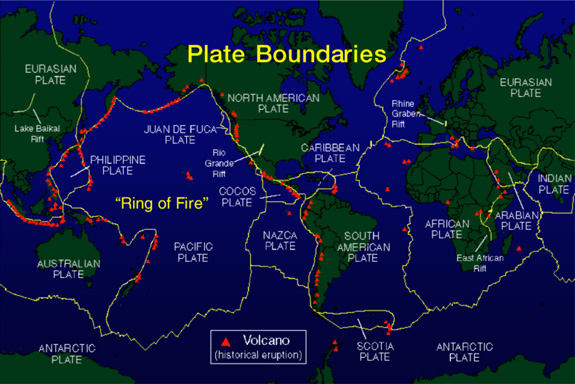
\includegraphics[width=4in]{plates.jpg} 
   \caption{Geothermal systems and plate boundaries}
   \label{fig:example}
\end{figure}

\\
A geothermal field is a geographical area with geothermal activity at the earth surface  \cite{Ax-Production08}. All hydrological systems directly related to geothermal resources such as fractures zone, heat source, aquifers etc... constitute the geothermal system. The geothermal reservoir is the permeable and hot part of the system \cite{Ax-Production08}.
Geothermal systems are classified on the basis of temperature (enthalpy) and their geological setting. 

\subsection{Classification based on temperature}
On the basis of temperature, geothermal systems can be classified as high temperature systems and low temperature systems. The temperature is at least $200\,^{\circ}{\rm c}$ in high temperature systems, while low temperature systems are characterised by temperature below $150\,^{\circ}{\rm c}$ \cite{Ax-Production08}.  The heat source in high temperature systems is often a hot intrusive magma, formed by incomplete melting of the upper mantle and the crust. High temperature systems are generally situated in volcanic regions. The heat source in low temperature systems, is the hot crust heated by radioactive elements.

\subsection{Classification based on geological formation}
On the basis of their geological setting, conventional geothermal systems can be classified as volcanic systems, convective systems, sedimentary systems, Engineered Geothermal Systems (EGS) and shallow geothermal systems \cite{Ax-Production08}.\\
\\
\emph{Volcanic systems} are located within or in the proximity of volcanic complexes. They  are high temperature systems and two phase flow (liquid and steam). The flow of water in volcanic systems is controlled by permeable fractures and fault zones  \cite{Ax-Production08}. The heat sources are hot intrusions or magma \cite{Ax-Production08}. \emph{Convective systems} are often situated outside volcanics complex and are predominantly low temperature systems. Characterised by highly fractured rocks heat is transferred within a convective system through convection cells. \emph{Sedimentary systems} are located in sedimentary basins characterised by permeable sedimentary layers. Heat is transfer mainly through conduction \cite{Ax-Production08}. An \emph{engineered geothermal system} generate geothermal energy without the need for natural convective hydrothermal resources. Through hydraulic stimulation, high pressure cold water is injected into the system, to enhance permeability in the naturally fracture rock. \emph{Shallow geothermal systems} refer to the thermal energy stored near the surface of the earth crust. This energy is utilised through heat pumps. \\
\\
Recently abandoned oil and gas wells or dry wells have been investigated for possible sources of geothermal energy.
Abandoned oil and gas wells are wells that ceased or never produced oil and gas. They can be as deep as 6000 $m$ \cite{Cheng2013}
In most geothermal project the cost of drilling can be as high as 50 $\%$ of the total project cost \cite{Bu2012}. By using abandoned oil and gas wells, the cost of geothermal energy production is reduced significantly. To produce geothermal energy from abandoned oil and gas wells, a double pipe heat exchanger is inserted into a well see Figure \ref{fig:ex}. \\
\begin{figure}[htbp] %  figure placement: here, top, bottom, or page
   \centering
   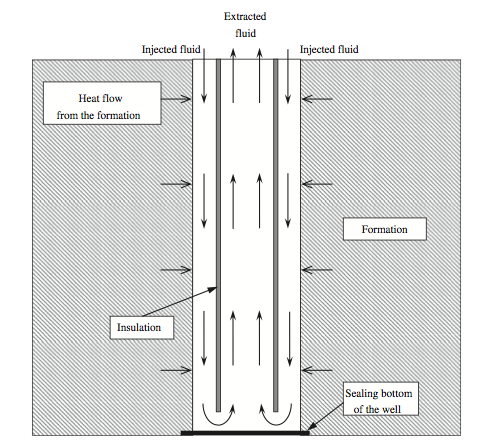
\includegraphics[width=4in]{doublep.png} 
   \caption{Diagram of a double pipe heat exchanger}
   \label{fig:ex}
\end{figure}
A working fluid is injected in one orifice of the heat exchanger. Due to the natural geothermal gradient, the fluid is heated by the geological formation. The recover geothermal energy depends on the flow rate of the injected working fluid and the geothermal gradient \cite{Bu2012, Cheng2013}. Computational simulation indicates that the fluid temperature can be around $130\,^{\circ}{\rm c}$ or more \cite{Bu2012}. Organic fluid such as isobutane can be used as working fluid. Due to their low boiling point they are easily converted into high temperature steam \cite{Cheng2013}.\\

%Geothermal energy from abandoned oil and gas wells is generated in a controlled environment. In the latter injected fluid in the geological formation can induce micro seismicity. On the other hand in abandoned oil and gas well, the fluid flow in a heat exchanger, reducing any risk of environmental hazards.
%%%%%%%%%%%%%%%%%%%%%%%%%%%%%%%%%%%%%%%%%%%%%%%%%%%%%%%%%%%%%



\subsection{Geothermal resource assessment methods}
Geothermal engineering is a multidisciplinary field of study. It includes numerical simulation, geophysics, geology and chemistry. The purpose of geothermal reservoir engineering is to estimate reservoir properties and production potential, simulate production response and estimate the size of geothermal resources. It plays a key role in resource management. Assessment methods in geothermal reservoir engineering are divided into two: Volumetric assessment method and dynamics assessment method \cite{Gudmundsdottir2012}. Volumetric assessment methods are used in the the first stage of a geothermal project and should be included in conventional geothermal monitoring programs \cite{Axelsson2008, Gudmundsdottir2012, Isor}. Volumetric method plays an integral role in geothermal resource management \cite{Axelsson2008}. It includes the use of geological, geophysical and chemical methods. Data from volumetric methods can be used to construct a conceptual model of the reservoir. The conceptual model is a descriptive model of the system. It incorporates the essentials physical features of the system such as heat sources, hot springs, permeable zones, boundary condition, recharge zones etc \cite{Osul01}. The conceptual model provides an estimate of the reservoir size and describes flow pattern within the system. It is the foundation for a successful numerical simulation. Volumetric method plays a key role during production. Dynamical methods includes simple analytical methods, details numerical simulations and lumped parameters modelling \cite{Gudmundsdottir2012}. A combination of volumetric methods and numerical simulation should enhance the reliability of mathematical model of geothermal systems \cite{Axelsson2000}


\subsubsection{Volumetric assessment methods}
\textbf{\underline{Geological methods}}\\
The most widely used method is geological mapping. It goal is to study the viability of a geothermal project. It includes geothermal surface manifestation mapping, surface petrology, mineralogy, lithology, tectonic. It also plays an import role in advanced stages of the project in well siting and well design. A map of surface thermal manifestation such as hot spring, mud pots and warm group can reveal if the geothermal field is active of extinct \cite{Isor}. \\
\\
\textbf{\underline{Geophysical methods}}\\
Geophysical methods are import part of geothermal resource assessment. Physical parameters such as density, resistivity and magnetism of the rock are measured. Gravity survey is used to measure the density variation, which can reveal dense intrusions.
Magnetic measurement can give information about dikes. Seismic surveys and seismic monitoring reveals fracture zones at depth \cite{Isor}. Gravimetric measurements may reveal tectonic features in the reservoir \cite{Isor}. Micro gravity monitoring can provide information on the net mass balance of the reservoir (difference between mass withdrawal and the recharge of water) \cite{Axelsson2000}. Mass balance from enlarging steam zones may also be seen from gravity monitoring \cite{Axelsson2000}.  Mass balance effect of reinjection may be detected by gravity monitoring \cite{ Axelsson2000}. Resistivity surveys reveals temperature distribution of the system and might help delineate cold fresh water inflow into the geothermal system \cite{Axelsson2000}. The commonly used resistivity survey are Transient ElectroMagnetic (TEM) and MagnetoTelluric (MT) sounding \cite{Isor}. 
\\
In TEM survey current is generated in a big loop laying on the ground. By induction the current produces a magnetic field in the ground. By turning off the current abruptly, the varying magnetic field in the ground induce a current. This current is used to map the resistivity structure of the upper most $1$ $km$ of the geothermal system \cite{Isor}.
\begin{figure}[H] %  figure placement: here, top, bottom, or page
   \centering
   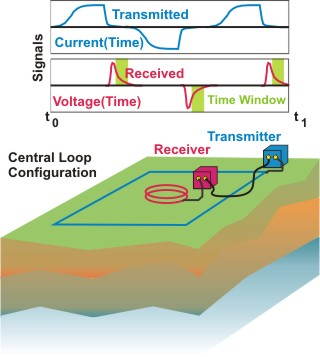
\includegraphics[width=2in]{tem.jpg} 
   \caption{TEM survey }
   \label{fig:tem}
\end{figure}
\\
The TM survey makes use of the natural fluctuation of the earth\�s magnetic field. By the principle of induction, the induced current in the earth is measured on the surface by two magnetics dipoles. Because the TM survey uses the natural magnetic field of the earth, it maps the resistivity structure of the geothermal system at greater depth, tens of $km$ \cite{Isor}.
\begin{figure}[H] %  figure placement: here, top, bottom, or page
   \centering
   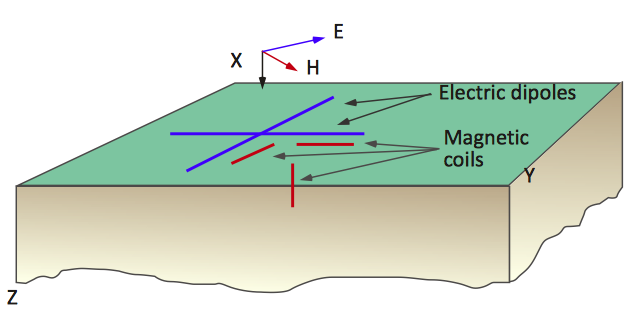
\includegraphics[width=4in]{tm.png} 
   \caption{TM survey}
   \label{fig:tm}
\end{figure}
 \\
\textbf{\underline{Chemical methods}}\\
Chemical composition of geothermal fluid (steam and water) can reveal the temperature of the reservoir. it plays an important role in anticipating corrosion and scaling in pipes and wells by identifying corrosive and scaling species. Chemical composition of the surface water reveals information about the recharge zone of a geothermal reservoir \cite{Isor}. Change in silica content of water production can be interpreted as inflow of cold water into the geothermal system \cite{Axelsson2000}.

\subsubsection{Dynamics assessment method}
\\
\textbf{\underline{Numerical simulation}}\\
Traditionally, conceptual models of geothermal systems are developed on the basis of information from various disciplines including geology, geophysics and geochemistry. Mathematical models are then applied to simulate the behaviour of the system using conceptual models \cite{Hagdu1995}.

On the basis of the conceptual model constructed from volumetric assessment methods, a careful mathematical model of the reservoir is constructed. Variables such as pressure, enthalpy, saturation, permeability, storage capacity are often simulated. A successful mathematical model is based on deep understanding of the physical and chemical processes of the system, the boundary condition, the fluid and rock properties, the location of sources and sinks  \cite{Osul01}. Fluid flow in geothermal systems can be approximated by flow in a porous medium. The flow is characterised both as single phase (water) with multi-component (carbon-dioxide and NaCl) or multi phase flow consisting of two phases, water and steam \cite{Hagdu1995}.
\\
Geothermal systems are modelled in terms of conservation of mass, momentum and energy. A complete model of the system should incorporate the flow of fluid in the reservoir and the production/reinjection wells \cite{Hagdu1995}. The general conservation equations for simulating two phase  flow in a geothermal reservoir are given by Grant \cite{Grant-Re82}:\\
\\
\textbf{Conservation of mass}
\begin{equation}
\phi\frac{ \partial  }{\partial t} \left ( \rho_{l}S_{l}f_{l}+  \rho_{g}S_{g}f_{g}   \right)+\nabla\cdot( \rho_{l}u_{l}f_{l}+ \rho_{g}u_{g}f_{g})+q_{m} = 0
\end{equation} 
where $\rho$, $S$  are the saturation and $f$ is the mass concentration of the chemical species in the fluid. $l$ and $g$ stand for liquid and gas (vapour). $u$ is given by equation (\ref{eq:cml},\ref{eq:cmg}). $q_{m}$ is the sink/source term $(kg)$ \\
\\
\textbf{Conservation of energy}
\begin{equation}
\phi\frac{ \partial  }{\partial t} \left ((1-\phi) \rho_{r}U_{r}+ \phi( \rho_{l}S_{l}U_{l} +\rho_{g}S_{g}U_{g} )   \right)+\nabla\cdot( \rho_{l}u_{l}h_{l}+ \rho_{g}u_{g}h_{g} -K\nabla T)+q_{E} = 0
\end{equation} 
$U$ is the internal energy, $h$ the enthalpy , $T$ the temperature, $K$ the heat conduction coefficient and $q_{E}$ the sink/source term $(J/m^{3}s)$.\\

%\clearpage
\textbf{Conservation of momentum}\\
The conservation of momentum is given by Darcys law. It describes a linear relationship between the fluid velocity and the pressure gradient relative to the rock:

\begin{equation}\label{eq:cml}
u_{l} = -\frac{kk_{rl}}{\mu_{l}}\nabla (P_{l}-\rho_{l}gz)
\end{equation}

\begin{equation}\label{eq:cmg}
u_{g} = -\frac{kk_{rg}}{\mu_{g}}\nabla (P_{g}-\rho_{g}gz)
\end{equation}
$k$ is the absolute permeability, and $k_{rl}$ and $k_{rg}$ are the relative permeabilities of the rock to the liquid and vapour phase respectively. The above equations hold assuming that capillary pressure effects are neglected.\\
\\

The steady state equation governing fluid flow in a vertical geothermal well is given by the mass, momentum and energy equation 
\cite{Bjornsson1987}
\begin{equation}
\frac{\partial m}{\partial z} = 0
\end{equation}

\begin{equation}\label{eq:cm}
\frac{\partial P}{\partial z}-\left(  \left( \frac{\partial P}{\partial z} \right)_{f}+ \left( \frac{\partial P}{\partial z} \right)_{a} + \left( \frac{\partial P}{\partial z} \right)_{p}     \right) = 0
\end{equation}

\begin{equation}\label{eq:ce}
\frac{\partial E}{\partial z}\pm Q= 0
\end{equation}

where $Q$ is the heat flow and $\left( \frac{\partial P}{\partial z} \right)_{f}, \left( \frac{\partial P}{\partial z} \right)_{a}, \left( \frac{\partial P}{\partial z} \right)_{p}$
are the pressure drop due to frictional, acceleration and potential forces along the well respectively. They are given respectively by

\begin{equation}\label{eq:f}
\left( \frac{\partial P}{\partial z} \right)_{f}= \varphi^{2}\left(    \frac{f_{lo}G^{2}}{4r_{w}\rho_{l}}   \right)
\end{equation}

\begin{equation}\label{eq:a}
\left( \frac{\partial P}{\partial z} \right)_{a} = G(xu_{g}+u_{l}(1-x))
\end{equation}

\begin{equation}\label{eq:a}
\left( \frac{\partial P}{\partial z} \right)_{p} = (\rho_{m})g
\end{equation}

$u_{l}$ and $u_{g}$ are the liquid and steam velocity, $\varphi^{2}$ is the two phase multiplier introduced by Martinelli and Nelson:
\begin{equation}
\varphi^{2} = 1+\left(\Gamma^{2}-1\right) \left(   B_{r}x(1-x)+x^{2}  \right)\nonumber
\end{equation}

\begin{equation}
\Gamma^{2} = \frac{\rho_{l}}{\rho_{g}} \nonumber
\end{equation}

\begin{equation}
B_{r} = B_{s}\left(         \frac{1}{2}\left(    1+\left(\frac{\mu_{g}}{\mu_{l}}\right)^{2}10^{-\frac{300\epsilon}{r_{w}}}   \right)\right)\nonumber
\end{equation}
$f_{lo}$ is the liquid friction factor and $B_{s}$ is given by Table \ref{table:bs}.

\begin{table}[H]

\centering
\caption{Different values of $B_{s}$ based on $\Gamma$ and $G$}
\label{table:bs}
\begin{tabular}{llr}

\toprule
%\multicolumn{2}{c}{Values $\Gamma, G, B_{s}$} \\
%\cmidrule(r){1-2}
$\Gamma$    & $G(\frac{kg}{m^{2}s})$ & $B_{s}$  \\
\midrule
$\leq9.5$      & $\leq 500$    & $4.8$      \\
\\
                       & $ 500\leq G \leq 1900$        & $\frac{2400}{G}$       \\
                       \\
                       &$\geq 1900$   &   $\frac{55}{G^{0.5}}$   \\
                       \\
  \hline   
  \\                                                                           
$9.5<\Gamma<28 $    & $\leq 600$     &  $\frac{520}{\Gamma G^{0.5}}$      \\
\\
                                        & $>600$     &  $\frac{21}{\Gamma}$      \\
                                        \\
  \hline    
  \\                             
$\geq 28$ &       &  $\frac{15000}{\Gamma ^{2}G^{0.5}}$     \\
\bottomrule
\end{tabular}
\end{table}

\begin{equation}\label{eq:energy}
E = m(   xh_{g} +(1-x)h_{l}+0.5(xu^{2}_{g}+(1-x)u^{2}_{l}) +g(L_{w}-z)       )
\end{equation}

For constant mass flow rate $m$ (\ref{eq:cm}, \ref{eq:ce}) can be solved for pressure $P$ and steam quality $x$ by using Newton method for system of nonlinear equations.\\
 \\
Equations governing the behaviour of a geothermal system can be solve numerically by various softwares.
Softwares for geothermal systems simulation fall into two categories: Reservoir and wellbore simulation software. The widely reservoir simulator are THOUGH and its family, STAR and TETRAD \cite{Pritchett1995, Pruess1999, Vinsome1993, Gudmundsdottir2012}. THOUGH family are designed to simulate the coupled transport of fluid, heat and chemical species for multi phase flow in porous and fracture media \cite{Pruess1999}. The conservation equations are discretised in space using the integral finite difference method \cite{Edwards1972, Narasimhan1976, Hagdu1995}.  The time derivative is discretised using a finite difference scheme (backward, forward, centered). Due to the fact that THOUGH is discretised using an integral finite difference method, it has the advantage of handling unstructured mesh as opposed to STAR and TETRAD. This makes THOUGH the facto reservoir simulation software \cite{Gudmundsdottir2012}\\
\begin{figure}[H] %  figure placement: here, top, bottom, or page
   \centering
   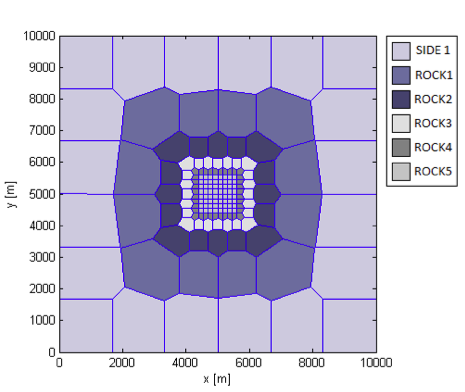
\includegraphics[width=4in]{mesh.png} 
   \caption{Unstructured mesh generated by THOUGH2. Taken from \cite{Gudmundsdottir2012}}
   \label{fig:example}
\end{figure}
The first wellbore softwares were designed to solve steady state conservation equation \cite{Gould1974, Gudmundsdottir2012}. The first simulator capable of handling unsteady state conservation equation was WELBORE designed by Miller \cite{Gudmundsdottir2012, Miller1980}. All these softwares solved the conservation equations from bottom to top along the well or vice versa, without incorporating the feed zones in the wells. The first software able to handle one feed zone was the software BROWN \cite{Bilicki1981, Gudmundsdottir2012}. HOLA was the first simulator capable of handling multiple feed zones in the well \cite{Bjornsson1987}.\\
\\

A successful geothermal systems simulation is based coupling empirical data and numerical simulation. The verification process map the measured data from the system to the result obtained from mathematical modelling. Verification is done through calibration \cite{Osul01}.  If the error between the measured and the calculated solution falls within an acceptable range, the simulation is a success. In this case the mathematical model represents a fairly good approximation of the system.
%\begin{figure}[H] %  figure placement: here, top, bottom, or page
%   \centering
%   %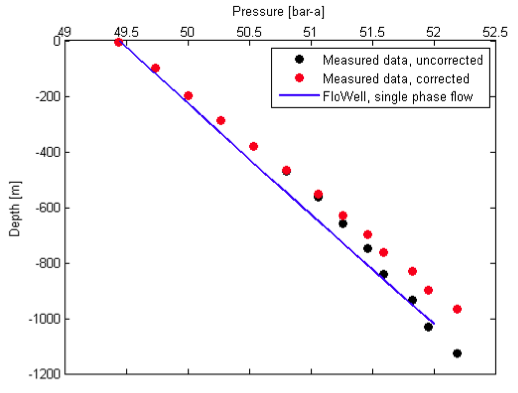
\includegraphics[width=2.5in]{val1.png} 
%      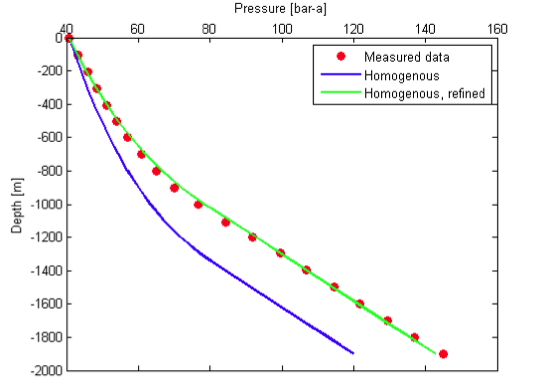
\includegraphics[width=4in]{val2.png} 
%   \caption{Verification process. Taken from (aldora)}
%   \label{fig:val}
%\end{figure}
Osulavan developed a general method of model calibration \cite{Osul01}. It consists of natural state modelling followed by history matching. In natural state modelling, the model is run for a long period of time to mimic the natural behaviour of the system. The simulated variables are compared with the measured field data. Some parameters of interest such as permeability structure, location of the heat source of the model are adjusted to obtain the minimum possible discrepancy between measured and simulated data. This step does not take into account the production history of the system. For system with production history, the measured behaviour of the geothermal field is matched with the simulated behaviour in response to production \cite{Osul01}. \\
\\
\textbf{\underline{Lumped parameters modelling and analytical method}}\\

A lumped parameter modelling software was designed by Axellsson to simulate the pressure change in a low temperature geothermal well \cite{Ax-Simul-Lump89}. The methods consist of approximating the permeability and the storage capacity of the reservoir by plumped parameters. By using inverse modelling the analytical response of the reservoir is mapped with measured data. Simple analytical method can also be used to model fluid flow in geothermal reservoir. In  Chapter (3) a case study using a lumped parameter modelling approach is presented. In chapter 4 a simple analytical method is used to predicts the thermal front velocity of injected cold water in a hot single phase geothermal reservoir.

%%%%%%%%%%%%%%%%%%%%%%%%%%%%%%%%%%%%%%%%%%%%%%%%%%%%%%%%%%%%%%%


\section{Reinjection in geothermal systems}
\subsection{Historical background and advantages}
Reinjection in geothermal resource management consist of reinjecting the used geothermal water back into the reservoir. Water of different origins such as  surface water and sewage water  can also be reinjected \cite{Ax-R08}. It started as a way on disposing the wast water from geothermal energy utilisation \cite{Ax-R08}. The first recorded instance of injection of cold water into a high temperature reservoir is in Ahuachapan field in El Salvador in 1969 \cite{Ax-R08, Stefansson1997}. At the same time a long term reinjection was used  successfully in the Dogger limestone reservoir located in the Paris basin \cite{Ax-R08}.  The Dogger reservoir stretching $150000 km^{2}$ is mainly used for district heating. The production and reinjection wells are separated by a distance of about $1km$. The reinjection scheme in the Paris basin lasting $30$ to $40$ years has indicated no significant cooling of the reservoir due to cold water injection \cite{Ax-R08}.
In 1970, operators in the Geyser geothermal field started to inject the steam condensate, and realised that this process increased the reservoir performance \cite{Ax-R08}. Since then reinjection has been an integrant part of resource management in the Geyser field. It was latter observed that due to injection, the decline of electrical production in the geyser was considerably slow \cite{Ax-R08, Stark2005}.
\\
In Italy reinjection started in 1974 at Lardelerollo field as a means to dispose the steam condensate \cite{Ax-R08, Capetti1995, Stefansson1997}. Long term production history has revealed that since reinjection started, steam production along with pressure have increased in the Lardelerollo geothermal field \cite{Ax-R08, Stefansson1997}, See Figure \ref{fig:lard}. 

\begin{figure}[H] %  figure placement: here, top, bottom, or page
   \centering
   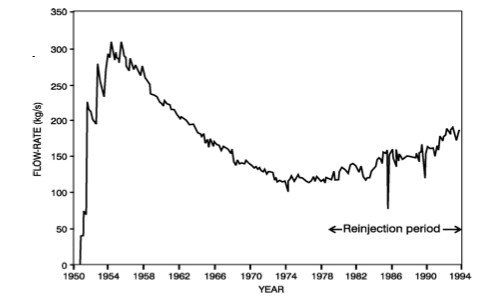
\includegraphics[width=4in]{lard.png} 
   \caption{Flow rate history at the Lardelorro field \cite{Capetti1995}. Taken from \cite{Ax-R08}}
   \label{fig:lard}
\end{figure}
 Reinjection sarted in Iceland in 1997 at the Laugaland low temperature field in north Iceland \cite{Axelsson2000}. In the Laugaland geothermal system 20 to 20$\%$ of the extracted mass are reinjected \cite{Axelsson2000, Ax-R08}. In the Hofstadir geothermal system in West Iceland reinjection started in 2006. About 40 to 50$\%$ of the extracted mass are reinjected back into the system \cite{Ax-R08}. Due to the low chemical content in most Icelandic geothermal field and the good recharge of water, reinjection started relatively late in Iceland \cite{Ax-R08}. Now reinjection is practiced in most of the hight temperature field in Iceland. It is estimated that the number of geothermal field in which reinjection is a part of resource management is likely more than 60 \cite{Ax-R08}. \\
 \\
 Reinjection is a vital part of an Enhanced Geothermal System (EGS) \cite{Ax-R08}. An EGS is a man made reservoir, created where there is hot rock but insufficient or little natural permeability or fluid saturation. About 80 to 90$\%$ of the energy of a geothermal reservoir is stored in the rock \cite{Ax-R08, Fowler05}. Therefore in an EGS, fluid is injected into the system at a sufficient pressure to create a fracture network into the rock with sufficient permeability. A production well is drilled into the fracture network to intersect the created flow paths. 
 
\begin{figure}[H] %  figure placement: here, top, bottom, or page
   \centering
   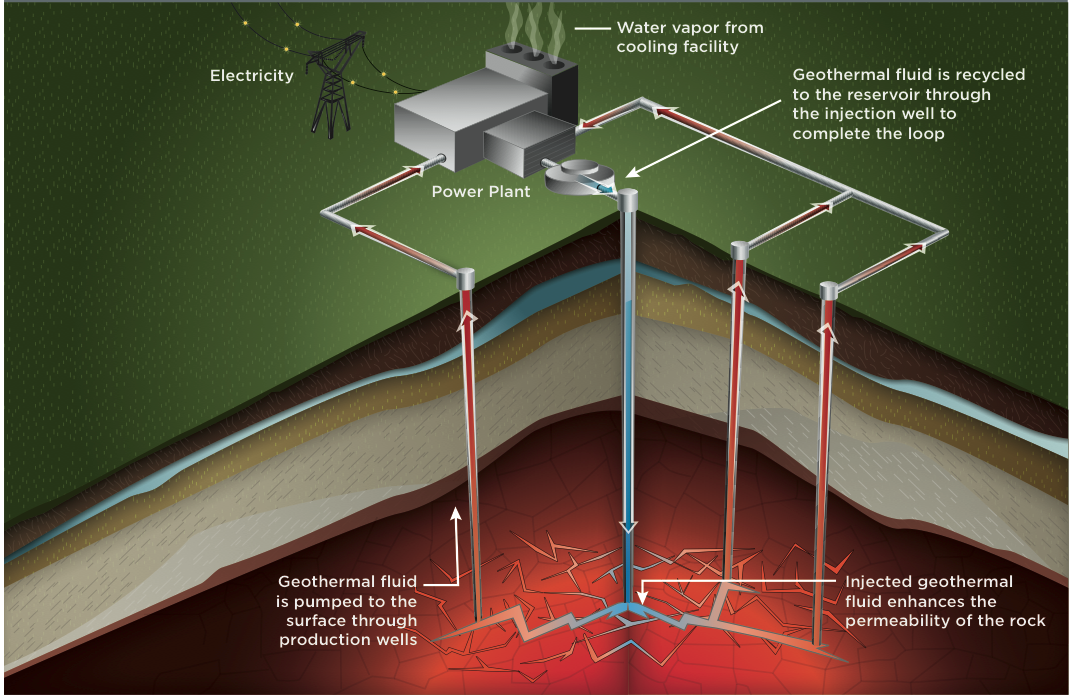
\includegraphics[width=5in]{egs.png} 
   \caption{schematic description of an EGS}
   \label{fig:egs}
\end{figure}

The production capacity of a geothermal system is controled by pressure response \cite{Ax-Production08}. During reinjection, the reservoir pressure is increased significantly, therefore reinjection increase the production capacity of the reservoir. As an environmental protection tool, it is a way of disposing the hight chemical content of geothermal wast water. It mitigates surface subsidence and maintains the integrity of surface activities \cite{Ax-R08}.\\
Reinjection can however affect the lifetime efficiency of the reservoir.  The lifetime efficiency of a reservoir can be defined as the ratio of the heat produced over it life time to the total available heat content of the reservoir \cite{Sayantan2012}. It can written as

\begin{equation}
\eta = \frac{E_{r}}{E_{T}} \nonumber
\end{equation}

where $\eta$ is the efficiency, $ E_{r}, E_{T}$ are the heat produced by the reservoir over it life time and the total available heat content respectively. The injected water is generally colder than the reservoir rock and can intersect fractures to create a premature cold water inflow and cool down the reservoir and decrease the reservoir efficiency. Reinjection can create and reopen pre-existing fractures. If created or reopen fractures intersect a cold aquifer, cold water breakthrough can be induced into the reservoir. Due to a large amount of fluid being injected into the reservoir, pressure increase can cause rock to slip along pre-existing fractures and produce microseismic events. Silica scaling in high temperature system, carbonate scaling in low temperature system and corrosion in pipelines and injection wells can be problems associated with injection. clogging of acquirers next to injection wells in sandstone reservoir can also be a significant problem \cite{Ax-R08}.
To mitigate the problems associated with reinjection , a careful reinjection scheme must be designed. 

\subsection{Mitigating problems associated with reinjection}
The main goals of reinjection can be summarise as follow:\\
1) Counteract pressure decline due to production\\
2) Maximise the reservoir efficiency by increasing the heat production over the life time of the reservoir\\
3)Environmental protection scheme\\
\\
If the purpose is option 3, injection wells can be placed outside the main production field without any direct hydrological connection \cite{Ax-R08}. If the purpose of the reinjection scheme is option 1 and 2, the rejection wells must be located inside the main production reservoir, in between production wells or on the outskirts of the reservoir but still in direct hydrological connection \cite{Ax-R08}. To avoid premature thermal breakthrough and increase the efficiency of the reservoir through injection, the injection scheme must ensure the optimum distance between injection wells and production wells \cite{Ax-R08, Sayantan2012}. Thermal breakthrough have been observed in relatively few geothermal systems worldwide \cite{Ax-R08, Stefansson1997}.  In the Palinpinon geothermal system in the Philippines, thermal breakthrough occur about $18$ months after reinjection started. The temperature dropped by about $50\,^{\circ}{\rm c}$ over a period of $4$ years \cite{Ax-R08}. Tracer tasting can be done to locate  fracture zones, flow path and determine the thermal front velocity to predict any premature thermal breakthrough. Analytical method can also be used the determined thermal front velocity. In chapter 4, an analytical method to determine thermal front velocity is presented.

\subsubsection{Tracer testing}
Tracer tests are the most powerful tool for studying connections between injection and production wells and predict thermal breakthrough \cite{AxelssonF2001}. It involves injecting a chemical tracer into the geothermal system, and monitor its recovery through time at various points.The chemical tracer arrival time and the thermal breakthrough time are proportional by $2-3$ order of magnitude \cite{Ax-R08}. Therefore determining the tracer arrival time gives the thermal breakthrough time. Three types of tracer are commonly used in geothermal application: Radioactive tracers such as Iodine-125, Iodide-131, Tritium etc, Fluorescent tracer such as rhodamin WT, chemical tracer such as iodide, bromide etc \cite{Axelsson2005}.\\ 
Assuming that a tracer of mass $M$ is injected at $t=0$ with injection rate $q$ into a one dimensional channel with cross sectional area $A$, porosity $\phi$ and fluid density $\rho$, 

\begin{figure}[H] %  figure placement: here, top, bottom, or page
   \centering
   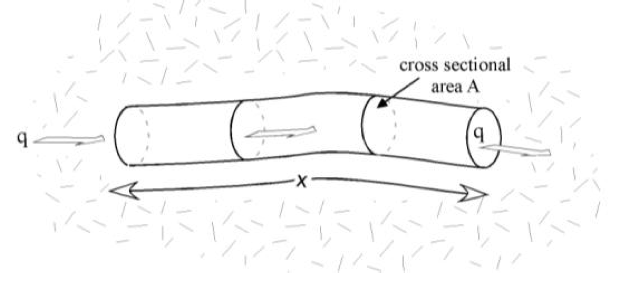
\includegraphics[width=4in]{chanel.png} 
   \caption{One dimensional flow channel connecting injection well and production well \cite{Axelsson2005}}
   \label{fig:example}
\end{figure}

The concentration $C$ of the tracer is modelled by \cite{Axelsson2005}:
\begin{equation}\label{eq:t}
\frac{\partial C}{\partial t}+u\frac{\patial C}{\partial x}-D\frac{\partial^{2}C}{\partial x^{2}} = 0
\end{equation}
The theoretical response
\begin{equation}\label{eq:s}
C(t) = \frac{4M\pho}{Q} \frac{1}{2\sqrt{\pi Dt}}\exp\left(-\frac{x-4t}{4Dt}\right)
\end{equation}
is simulated with the tracer data to obtain the flow channel volumes $Ax\phi $ and the longitudinal dispersivity $\alpha_{L}$ \cite{Axelsson2005}. In equation (\ref{eq:t}, \ref{eq:s})  $ u = \frac{q}{\rho A\phi}$, $D=\alpha_{L}u$, $Q$ is the production rate of the production well.
\\
The software TRINIV included in the ICEBOX software package developed at Iceland geosurvey uses a non linear least squares fitting to simulate data and return the flow channel volumes and the dispersivity \cite{Axelsson2005}. Ones equation (\ref{eq:s}) is fully defined, the concentration profile $C(t)$ can be use to determine the arrival time of the tracer concentration. 
 




%----------------------------------------------------------------------------------------
